% This file is iccc.tex.  It contains the formatting instructions for and acts as a template for submissions to ICCC.  It borrows liberally from the AAAI and IJCAI formats and instructions.  It uses the files iccc.sty, iccc.bst and iccc.bib, the first two of which also borrow liberally from the same sources.

\documentclass[letterpaper]{article}
\usepackage{iccc}


\usepackage{times}
\usepackage{helvet}
\usepackage{courier}

% Packages maison
\usepackage{amsmath,amssymb} % For including math equations, theorems, symbols, etc
\usepackage{bm}
\usepackage{graphicx} % Required for including images
\graphicspath{{../Figures/}} % Set the default folder for images
\usepackage{prettyref}

\pdfinfo{
/Title (Formatting Instructions for Authors)
/Subject (Proceedings of ICCC)
/Author (ICCC)}
% The file iccc.sty is the style file for ICCC proceedings.
%
\title{The \textit{Live Orchestral Piano} : a conditional model for musical orchestration}
\author{L\'eopold Crestel, Philippe Esling\\
\'Equipe Repr\'esentation Musicales\\
Institut de Recherche et Coordination Acoustique/Musique\\
1 Place Igor-Stravinsky, 75004 Paris\\
leopold.crestel@ircam.fr, philippe.esling@ircam.fr\\
}
\setcounter{secnumdepth}{0}

\begin{document} 
\maketitle
\begin{abstract}
\begin{quote}
This paper introduces several statistical models for the automatic projective orchestration of a piano score. We evaluate the RBM, CRBM and FGCRBM models on a short-term frame-level predictive task well-known in time-series modelling. We show the limits of this evaluation for musical sequences, propose an alternative event-level based task, and evaluate the same models in this new framework. We eventually introduce a \textit{Max/MSP} based system that perform in real-time the orchestration of notes played on a midi keyboard.
\end{quote}
\end{abstract}

\section{Introduction}
% Orchestration classique
%% Musical orchestration : why is it so hard ?
\textit{Musical orchestration} is the subtle art of writing musical pieces for the orchestra, by combining the different instruments in order to create a particular sound. A classic exercise, which has actually been used by many famous composer as writing method, consists in two steps. An harmonic, melodic, and rhythmic structure is first written in the form of a piano score (or equivalently any polyphonic instrument). This structure is then projected on an orchestra, by spreading the harmonic, melodic and rhythmic structure over the different instruments. This second step, the mapping from a piano score to an orchestral score, is often referred to as \textit{projective orchestration}. Given the number of different instruments in a symphonic orchestra and their respective range of notes, one can foresee the large number of possible combination implied.

Beside this combinatorial problem, the resulting sound of an even simple instrumental mixture is particularly difficult to predict, especially its emerging timbre. Several attempts to mathematically characterize the timbre as a set of spectro-temporal descriptors have outputted the complex non linear behaviours involved. Furthermore, an interesting orchestration will generally not simply be the allocation of the notes written on the piano score over the different instrument but will imply extension of the harmony and doubling some note with the octave. Eventually, orchestration is often referred to as the art of manipulating instrumental timbres, which lacks of both proper musical notation and a precise mathematical definition.
Those difficulties have probably been a major obstacle toward the construction of a theory of orchestration. Then it remains a mainly empirical discipline, taught through the observation of already existing orchestrations (\cite{piston-orch}).

Our objective is to build a system able to automatically perform projective orchestration. Its input is then a piano score and its output an orchestra score. To our best knowledge, this problem has never been tackled before.

% Inference stat for orchestration
If our inability to define precise rules discard the construction of a \textit{handmade} rule based system, it does not mean that underlying regularities could not be extracted. The classic and romantic repertoires contain a large number of examples of projective orchestration (e.g. the piano reduction by Liszt of the symphonies of Beethoven, \textit{les tableaux d'une exposition}, a piano piece from Modest Moussorgsky orchestrated by Ravel). Using statistical inference on a corpus constituted by piano scores and their projective orchestration by famous composers seems to be a promising lead. We believe that an appropriate statistical model would be able to extract the complex correlations that  occur along both time pitch and instrument dimensions and that human are unable to fully understand.

% Only symbolic justification (ici ou dans le texte ???)
%It has been pointed out that orchestration is art timbre blablablabl Besides, we hypothesize that in the purely symbolic information contained in the score written by composer lie knowledge about acoustic properties. Considering that all the information about instrumental mixtures is contained at a symbolic level is a strong assumption, but not a non-sense since those examples have been composed based on a certain knowledge.

\begin{figure}
\centering
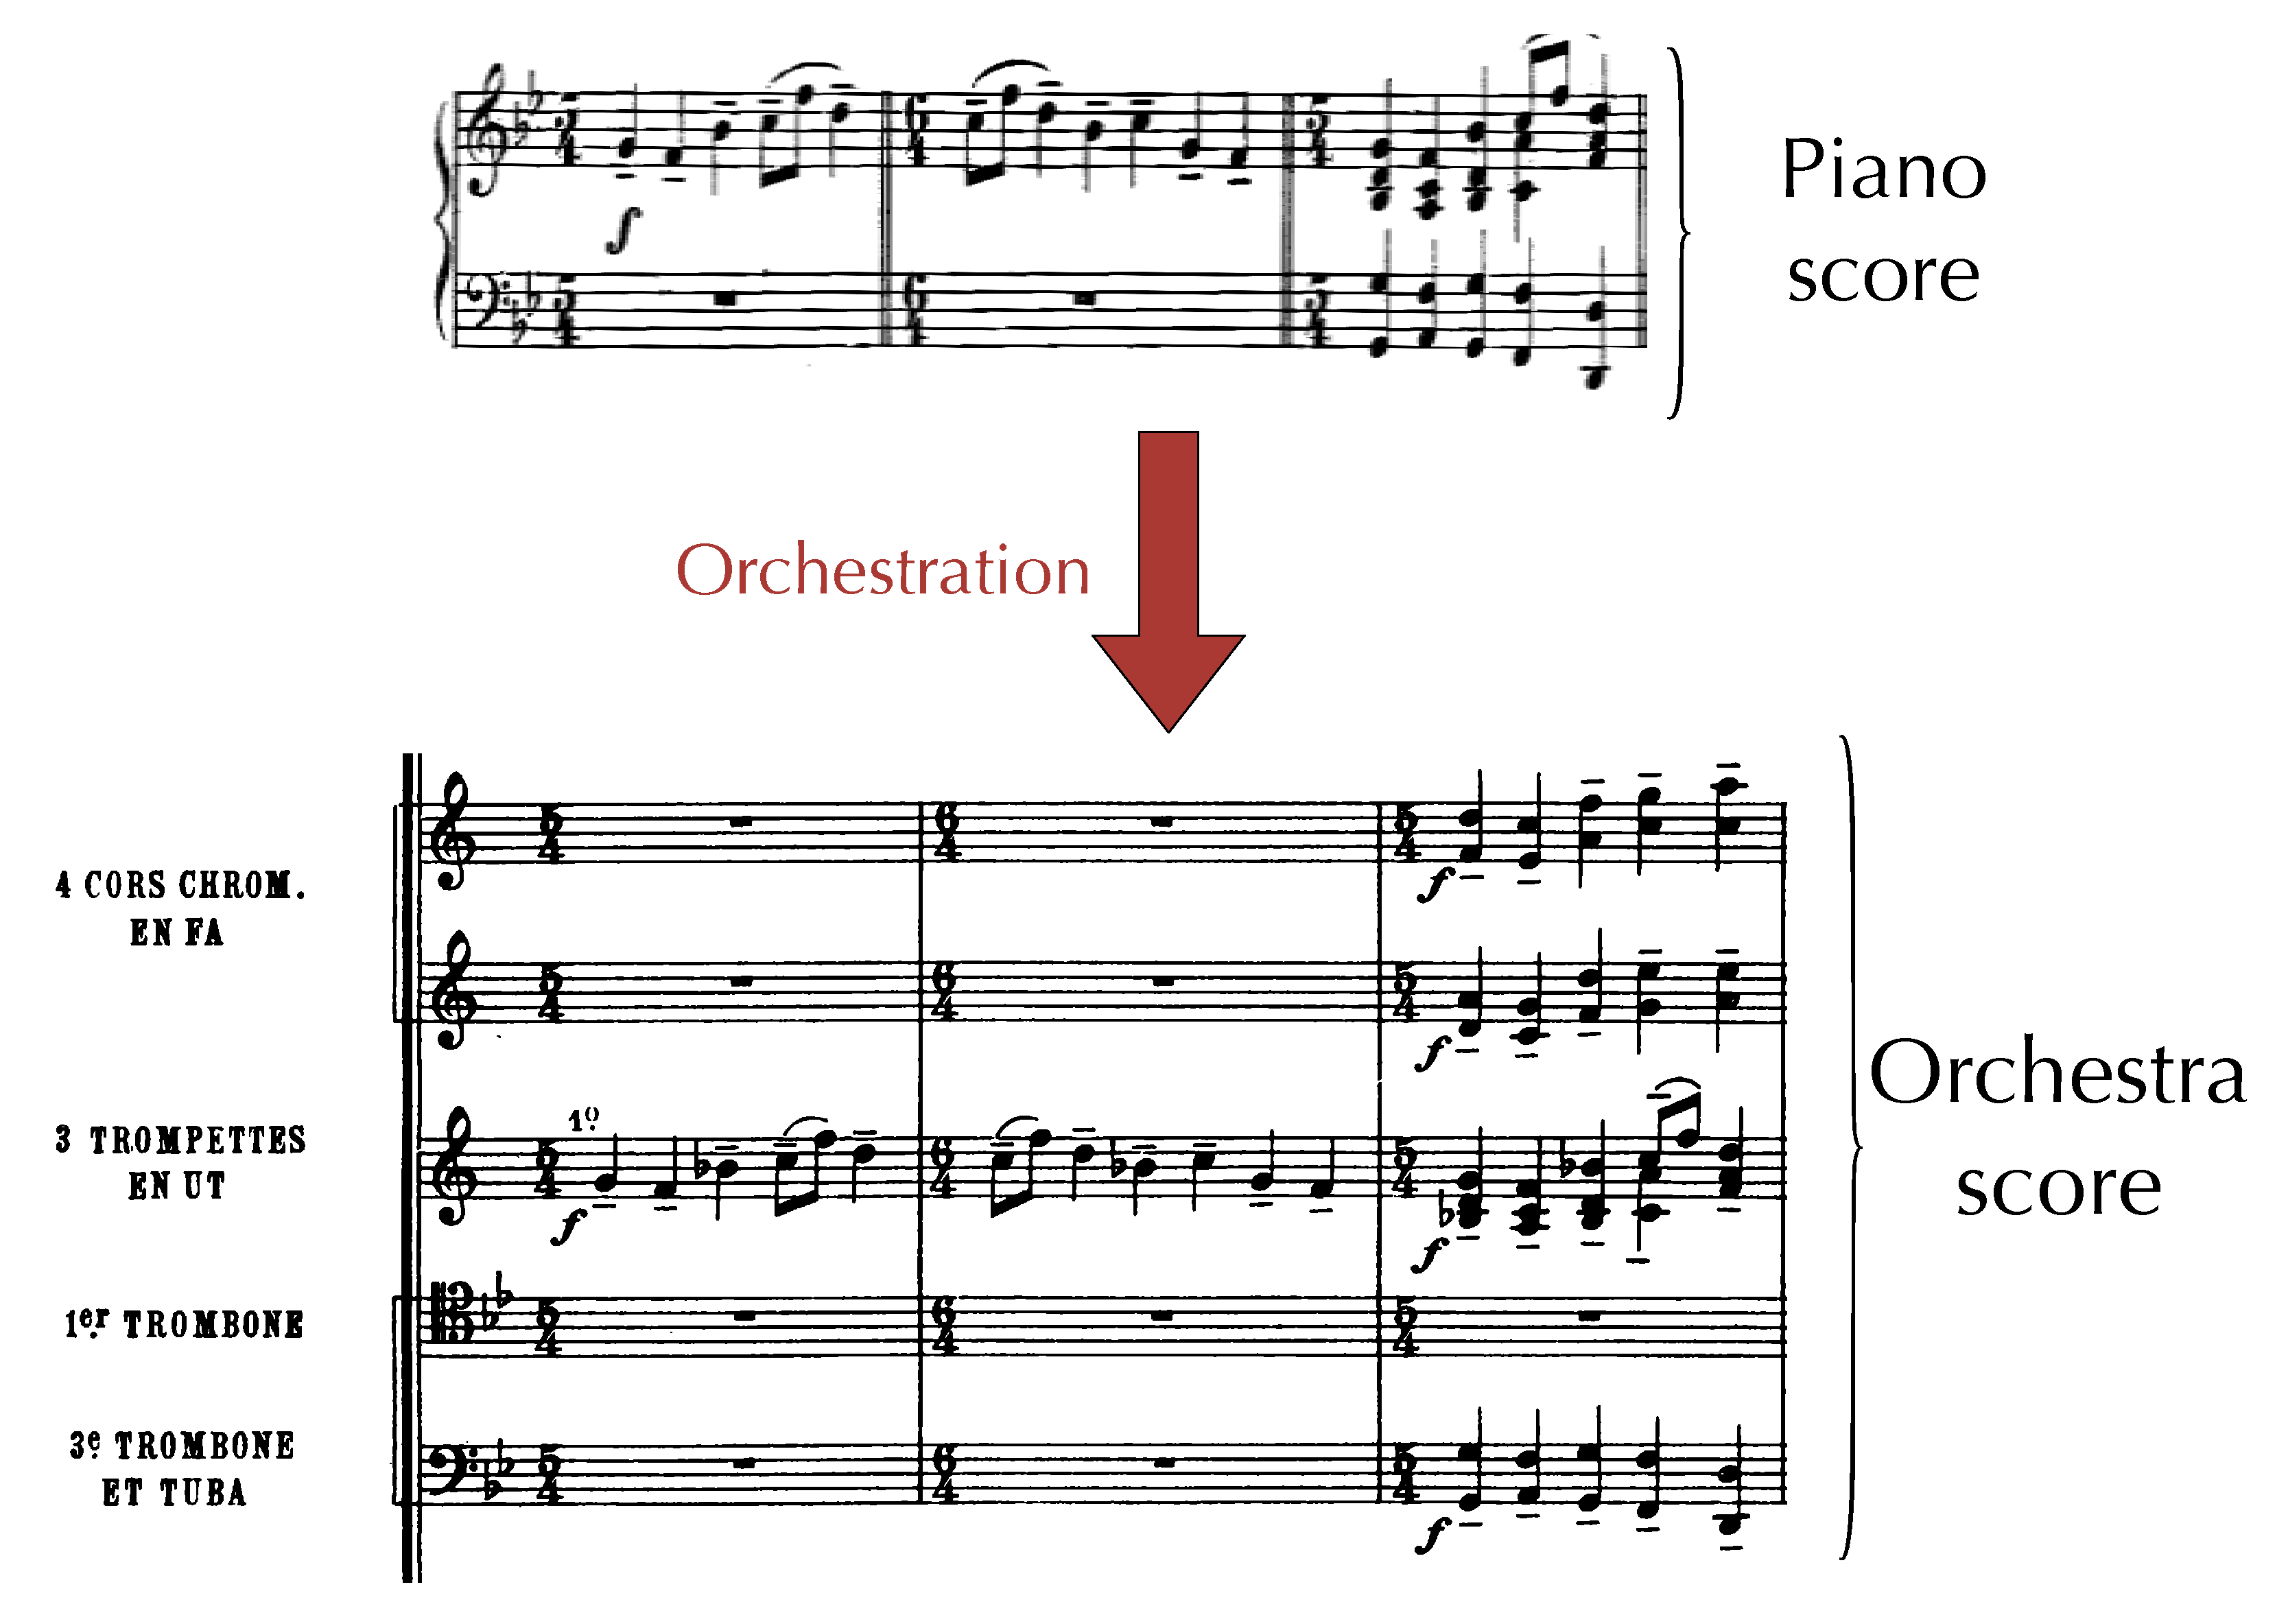
\includegraphics[scale=0.13]{orch}
\caption{\textit{Projective orchestration}. A piano score is extended (projected) on an orchestra. For one piano score, many acceptable orchestration exist. Our hypothesis is that a piano score is strongly correlated to any of the orchestration that could be produced from this piece.}
\label{fig:orch}
\end{figure}

%Stat inf ?
Statistical inference refers to methods which suppose that a set of data has been drawn from a probability distribution. The objective is to deduce properties of this underlying distribution, by observing a subset of those data. In our case, the objective is to infer rules of orchestration by observing pieces written by famous composers (experts). Inferring properties about this underlying probability distribution is called the \textit{learning} phase.
In our context, it can be seen as trying to find the correlations between a piano score and an orchestral score observed in the training set. Note that for one original piano score, many different orchestrations are acceptable with no objective criterion to rank them. The probabilistic framework perfectly fits this diversity of solution.
Statistical inference covers a wide range of domains. Among them, deep learning recently appeared as a most promising field in intelligence artificial and representation learning.

% Which model and why ?
To fully specify a statistical inference model, we need to specify a data representation, a probabilistic model and a training algorithm.
To represent the scores we used a piano-roll representation which is standard in computer music (see \prettyref{fig:pianoroll}). This is often referred to as symbolic information by contrast with signal information (recording of a performance). We evaluated two different probabilistic models : a conditional Restrictesd Boltzmann Machine (\textit{cRBM}) and a Factored Gated \textit{cRBM} (\textit{FGcRBM}) \cite{taylor2009factored}. Those two models can be trained by an algorithm called Contrastive Divergence (\textit{CD}) \cite{carreira2005contrastive}.
% Evaluation
Deriving an evaluation criterion for those three models is a requirement in order to select the optimal set of hyper-parameter for a given model and as a comparison between the models. A common criterion in statistical inference is the likelihood function of a dataset. However, this function is intractable for those models (see \prettyref{sec:state_of_the_art}). Hence, we propose an orchestral inference task which is inspired by the short-term frame-level predictive evaluation framework used in time series prediction. 
% Flaw 
In this framework, we evaluate the two previously introduced model along with baseline models (random generation, repeat of the previous frame and standard Restricted Boltzmann Machine (\textit{RBM})).
We show that this framework is heavily dependent on the quantization frame chosen to build the pianoroll and then propose an alternative framework in which the same models are re-evaluated.

% LOP
An interesting property of the \textit{cRBM} and \textit{FGcRBM} models is that their generative step is sufficiently fast for real-time application. We introduce \textit{LOP} (for \textit{Live Orchestral Piano}), the first system of real-time orchestration of a piano input.

This paper is organized as follows. Section 2 introduces the state of the art in conditional models : RBM, CRBM and \textit{FGCRBM} models are detailed. The orchestration projection task is presented in the section 3 along with an evaluation framework based on a frame-level accuracy measure. The introduced models are evaluated in this framework and compared with existing models. Section 4 introduces \textit{LOP}, the real-time \textit{projective} orchestration system. Finaly, Section 5 provides our conclusions and future works.

\section{State of the art}
\label{sec:state_of_the_art}
In this section, the three models evaluated in this contribution are detailed. The \textit{RBM}, the \textit{cRBM} and the \textit{FGcRBM} are presented by increasing level of complexity, each model adding a new \textit{degree of freedom} to the previous one.

\subsection{Restricted-Boltzmann Machine}
\begin{figure}
\centering
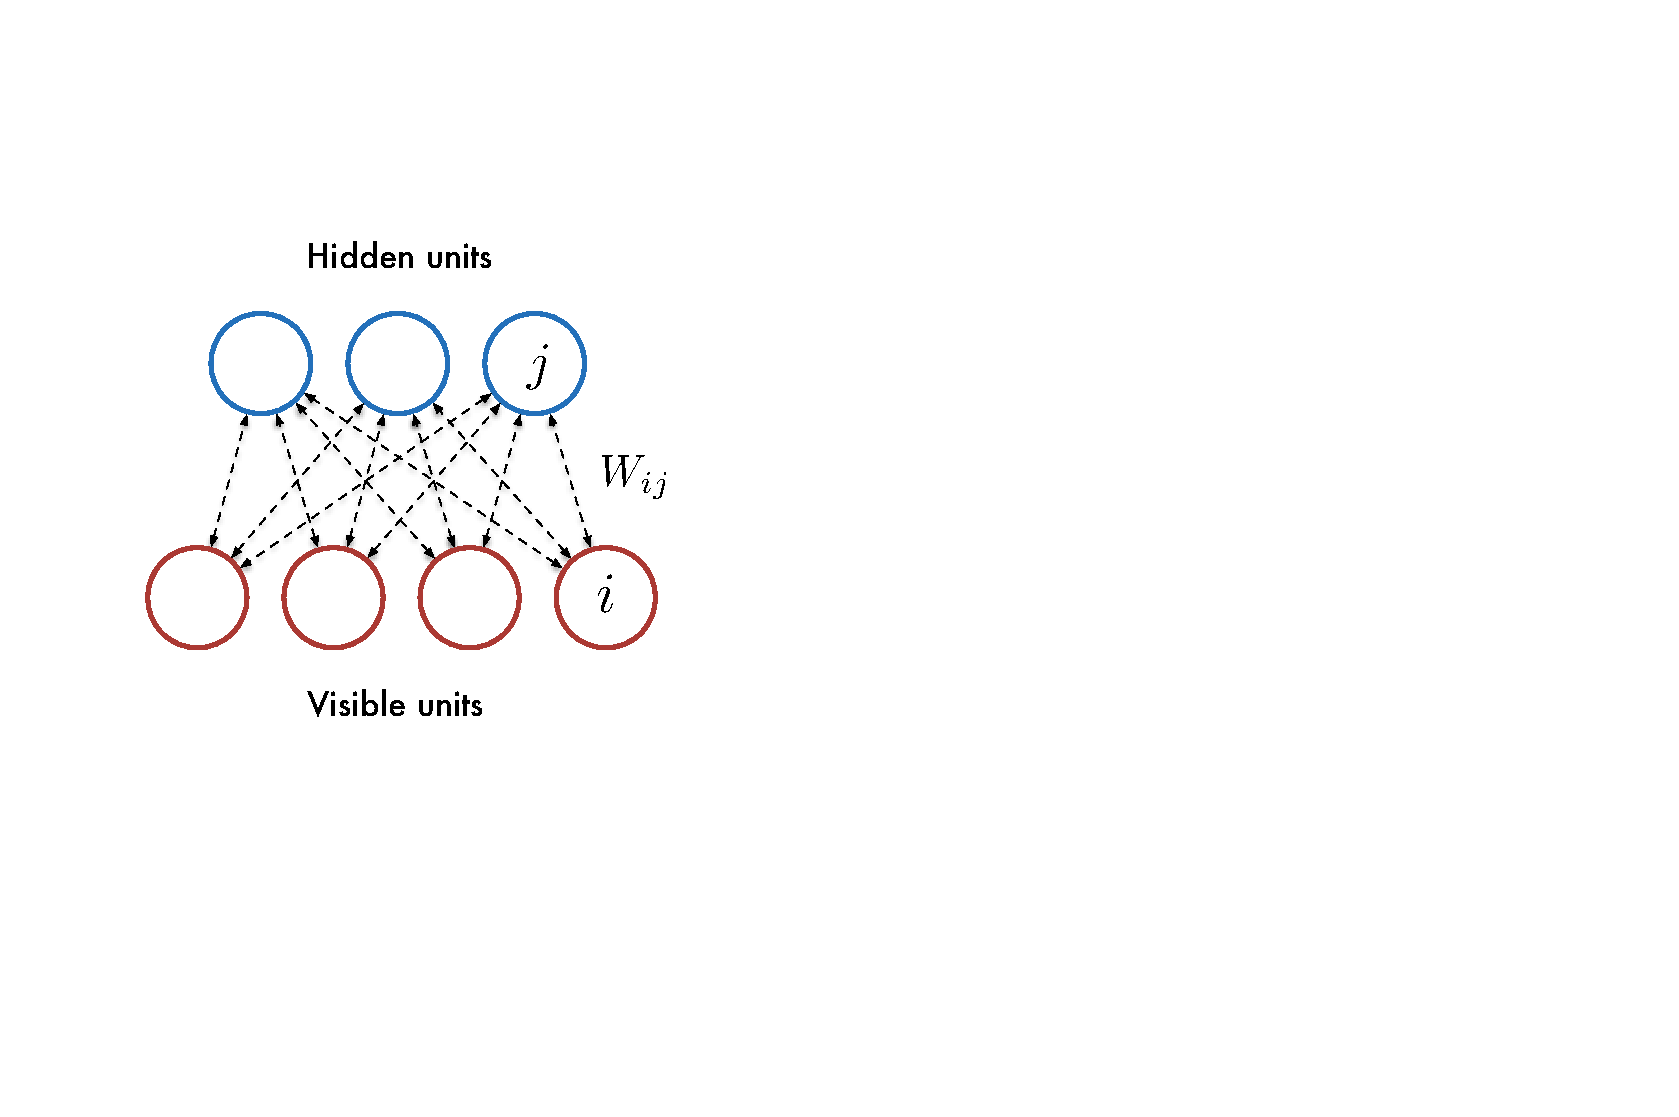
\includegraphics[scale=0.7]{RBM}
\caption{The \textit{Restricted Boltzmann Machine} (RBM) is defined by its units ($i$ or $j$) and weights ($W_{ij}$). Units are divided between visible units (4 units at the bottom) and hidden units (3 top-most). Weights and units define an energy function. Training an RBM consists in lowering the energy function around the example from a training set. Inference in this model is easy to perform since the hidden (resp. visible) units are independent from each others.}
\label{fig:RBM}
\end{figure}
\textit{RBM} \cite{hinton2006fast} is a graphical probabilistic model \prettyref{fig:RBM}. It is composed by a set of units, each representing a random variable. Links between those units represents conditional dependencies between those variables and are named \textit{weights}. The units are divided between visible, denoted by the vector $\bm{v} = (v_{1},...,v_{m})$, and hidden units, $\bm{h} = (h_{1},...,h_{n})$. Visible nits generally represent the observed data, and then have the same dimension as the vectors in the training set. Hidden units model explanatory unobserved factors.
Weights between units are denoted $W_{ij}$. The joint probability of the visible and hidden units is given by $p_{model}(\bm{v},\bm{h}) = \frac{\exp^{-E(\bm{v},\bm{h})}}{Z}$ where
\begin{equation}
\label{eq:likelihood}
E(\bm{v},\bm{h}) = - \sum_{i=1}^{m} a_{i} v_{i}  - \sum_{i=1}^{m} \sum_{j=1}^{n} v_{i} W_{ij} h_{j} - \sum_{j = 1}^{n} b_{j} h_{j}
\end{equation}
is the energy function associated to the model. $Z = \sum_{v,h}\exp^{-E(v,h)}$ is a normalizing factor to probability and is called the partition function. $\bm{\theta} = \left\lbrace \bm{W} , \bm{a} , \bm{b} \right\rbrace$ is the set of parameters of the network.

In this context, training a model on a set of data means that we want the distribution of the model ($p_{model}$) to be as close as possible to the hypothetical real distribution of those data ($p_{data}$). A commonly used criterion for training this model is to maximize the likelihood of the training set. The vectors from the training set $\mathcal{D}$ are designated by $\bm{v^{(l)}}$.
Instead of maximiazing the likelihood, minimizing the negative log-likelihood is often preferred as it simplify expressions :
\begin{equation}
\mathcal{L(\bm{\theta}|\mathcal{D})}  = \frac{1}{N_{\mathcal{D}}} \sum_{\bm{v^{(l)}} \in \mathcal{D}} - \ln \left( p(\bm{v^{(l)}}|\bm{\theta})\right)
\end{equation}
where $N_{\mathcal{D}}$ is the size of the dataset. 

The search for the minimum of a non-linear function can be tackled by using gradient descent \cite{bottou2010large}. The gradient of the negative log-likelihood of any vector from the training database $\bm{v}^{(l)}$ is given by
\begin{equation}
\begin{split}
- \frac{\partial \ln \left[ p(\bm{v^{(l)}}|\bm{\theta})\right]}{\partial \bm{\theta}} 
= 
\mathbb{E}_{p(\bm{h}|\bm{v^{(l)}})} \left[ \frac{\partial E(\bm{v^{(l)}},\bm{h})}{\partial \bm{\theta}} \right] 
- \\
\mathbb{E}_{p(\bm{v} , \bm{h})} \left[ \frac{\partial E(\bm{v},\bm{h})}{\partial \bm{\theta}} \right]
\end{split}
\end{equation}
It is interesting to note that this represent the difference between two expectations of the same quantity. The expectation on the left is referred to as the \textit{data-driven} term since it is an expectation over the distribution of the hidden units conditionally on a specific sample from the data distribution. The expectation on the right is referred to as the \textit{model-driven} term since it is an expectation over the joint distribution of the model.
Unfortunately this quantity is intractable because it involves a sum over all the possible configurations of the hidden (alternatively visible) units in order to compute the partition function \cite{Fischer2012}.

A training algorithm called \textit{CD} \cite{hinton2002training} rely on an approximation of this model driven term :
\begin{equation}
\label{eq:grad_log_like}
\begin{split}
- \frac{\partial \ln \left[ p(\bm{v^{(l)}}|\bm{\theta})\right]}{\partial \bm{\theta}}
\approx 
\mathbb{E}_{p(\bm{h}|\bm{v^{(l)}})} \left[ \frac{\partial E(\bm{v^{(l)}},\bm{h})}{\partial \bm{\theta}} \right] 
- \\
\mathbb{E}_{p(\bm{h} | \bm{v^{(l,k)}})} \left[ \frac{\partial E(\bm{v^{(l,k)}},\bm{h})}{\partial \bm{\theta}} \right]
\end{split}
\end{equation}
where $\bm{v}^{(l,k)}$ is obtained by running a k-step Gibbs chain. A Gibbs chain consists in alternatively sampling the hidden units knowing the visible units and the visible knowing the hidden \prettyref{eq:marginal_RBM}.
\begin{align}
\label{eq:marginal_RBM}
p(v_{i}=1|\bm{h}) &= \sigma \left( a_{i} + \sum_{j}W_{ij}h_{j} \right)\\
p(h_{j}=1|\bm{v}) &= \sigma \left( b_{j} + \sum_{i}W_{ij}v_{i} \right)
\end{align}
where $\sigma	(x) = \frac{1}{1+e^{-x}}$ is the \textit{sigmoid} function. Note that sampling from the marginal distribution is easy since visible units (respectively hidden units) are independent from each others. Hence, knowing the hidden units, all the visible units can be sampled in one step. This allows for a fast implementation of the sampling step through matrix calculus, known as \textit{block sampling}.
It has been proved \cite{bengio2009learning} that the samples we obtain after an infinite number of iteration will be drawn from the joint distribution of the visible and hidden units of our model. Approximations in running the Gibbs chain can be made by starting the chain from the same sample $\bm{v}^{(l)}$ used in the \textit{data-driven} term. This speed-up the convergence of the chain. A second approximation is to limit the number of sampling steps to a fixed number K. After evaluating the statistics of the distribution $\bm{h} \sim p(\bm{h}|\bm{v^{(l)}})$ and $\bm{v^{(l,k)}}$ and $\bm{h}\sim p(\bm{h}|\bm{v^{(l,k)}})$ from the Gibbs sampling chain, the parameters can be updated. The whole algorithm is called Contrastive Divergence-K (CD-K). In a \textit{RBM} the update rules are given by
\begin{align}
\Delta W_{ij} &= <v_{i}h_{j} >_{data} - <v_{i}h_{j} >_{model}\\
\Delta a_{i} &= <v_{i}>_{data} - <v_{i}>_{model}\\
\Delta b_{j} &= <h_{j} >_{data} - <h_{j} >_{model}
\end{align}

\subsection{Conditional RBM}
\begin{figure}
\centering
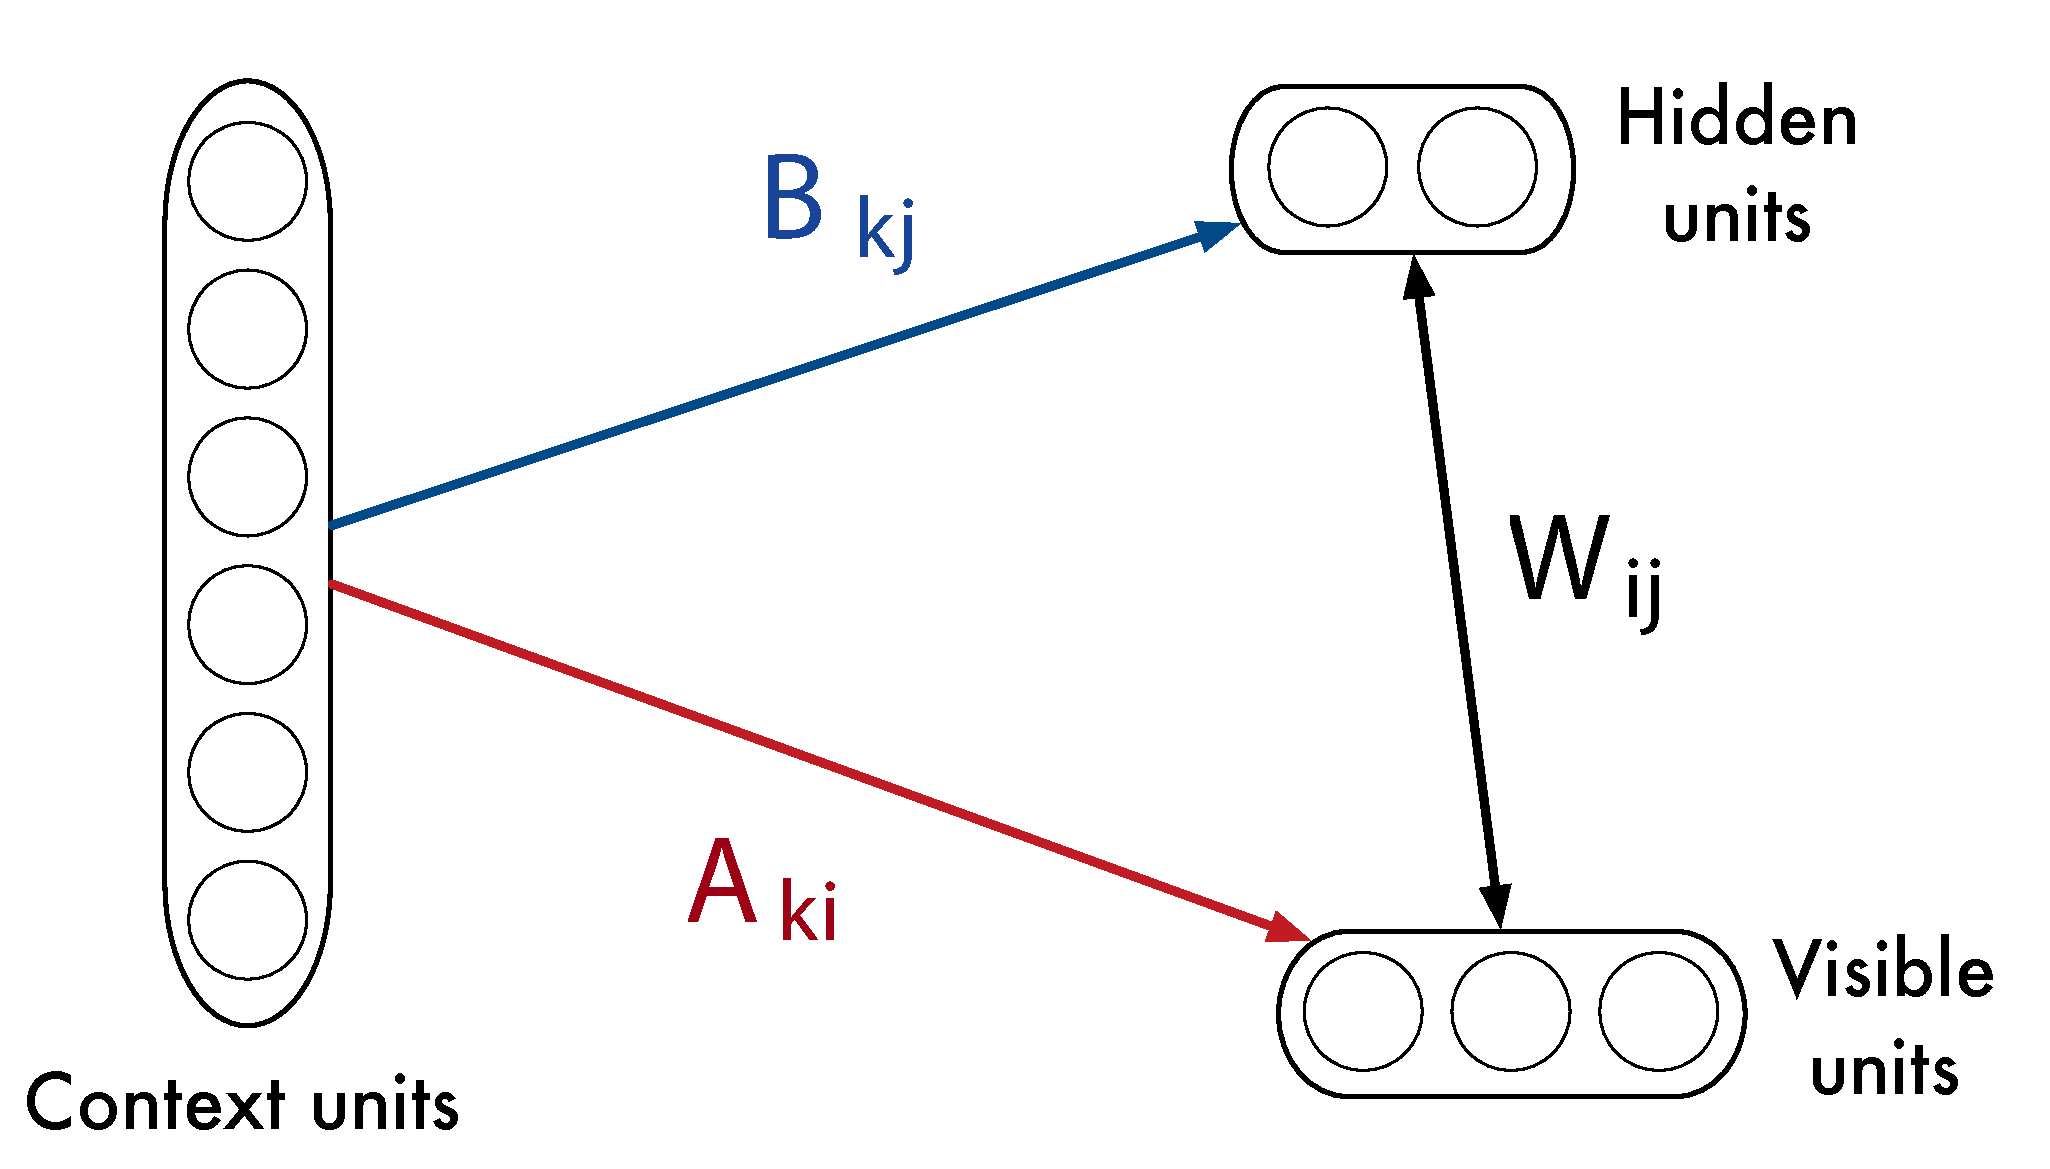
\includegraphics[scale=0.26]{CRBM_orchestration}
\caption{\textit{Conditional RBM} adds a layer of context units to the standard RBM architectures. Those context units linearly modify the bias of both visible and hidden units.}
\end{figure}
The Conditional \textit{RBM} model \cite{taylor2009factored} is an extension of the \textit{RBM} in which dynamic biases are added to the static biases of the visible and hidden units (respectively $\bm{a}$ and $\bm{b}$). This dynamic bias linearly depends on a set of units called context units $(\bm{x})$. In the context of time series, if the visible units represent a frame at time $t$, these context units can be used to model the influence over it of the recent past frames ($t-N$,...,$t-1$, where $N$ denotes the \textit{temporal order} of the model).
The energy function of the Conditional RBM is given by
\begin{equation}
\begin{split}
\label{eq:energy_CRBM}
E(\bm{v}(t),\bm{h}(t)|\bm{x}(t)) =  - \sum_{i} \hat{a}_{i}(t)v_{i}(t) - \\ \sum_{ij}W_{ij}v_{i}(t)h_{j}(t) - \sum_{j} \hat{b}_{j}(t)h_{j}(t)
\end{split}
\end{equation}
where the biases are defined by 
\begin{align*}
\hat{a}_{i}(t) &= a_{i} + \sum_{k}A_{ki}x_{k}(t)\\
\hat{b}_{j}(t) &= b_{j} + \sum_{k}B_{kj}x_{k}(t)
\end{align*}
We will refer to the matrices $\bm{A}$ and $\bm{B}$ as \textit{auto-regressive matrices}.

This model can be trained using CD, since the marginal probabilities of visible and hidden units are the same as the \textit{RBM}, simply replacing the static biases by dynamics ones.
The following update rules are unchanged for $\bm{W}$, $\bm{a}$ and $\bm{b}$, and are the following for the auto-regressive matrices
\begin{align}
\Delta A_{ik} 	&=<v_{i}x_{k} >_{data} - <v_{i}x_{k} >_{model}\\
\Delta B_{jk} 	&= <h_{j}x_{k} >_{data} - <h_{j}x_{k} >_{model}\\
\end{align}

\subsection{Factored Gated cRBM}
\begin{figure}
\centering
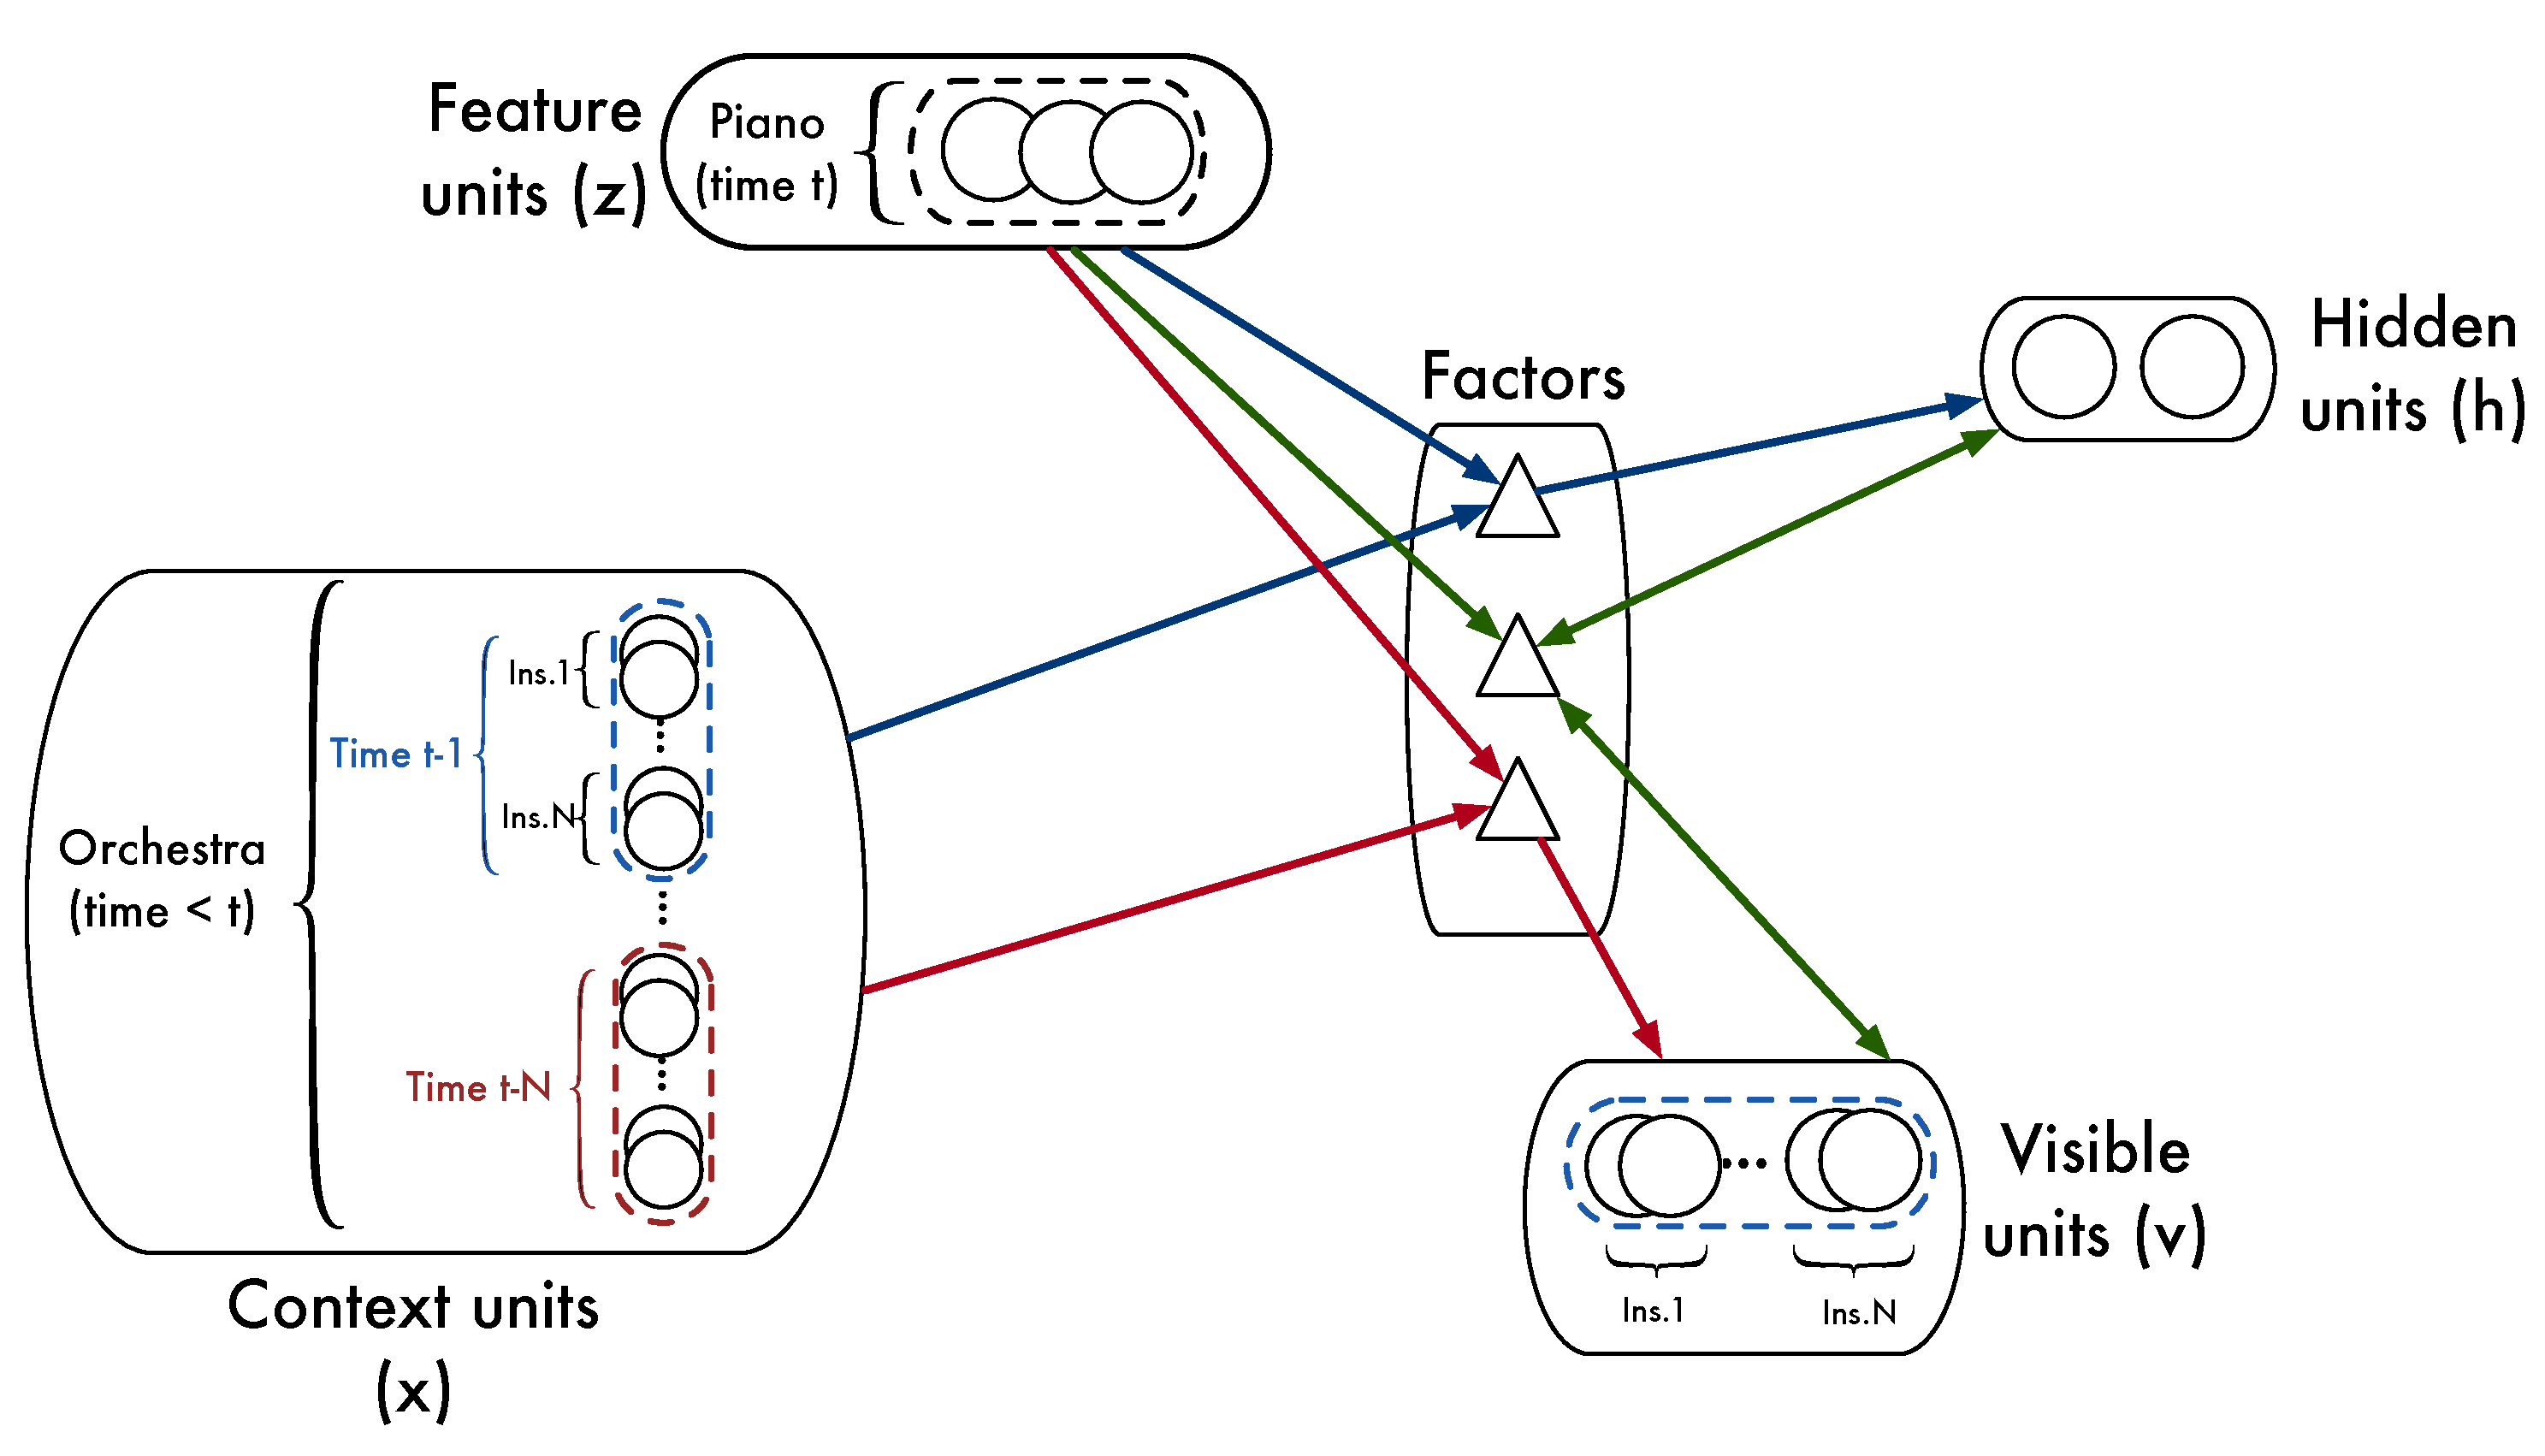
\includegraphics[scale=0.20]{FGCRBM_orchestration}
\caption{\textit{FGCRBM} model. The features units ($\bm{z}$) modify the energy landscape of the model through a multiplicative influence over the weights $\bm{A}$, $\bm{B}$ and $\bm{W}$. Here, the role of each unit in the context of orchestration is indicated.}
\label{fig:FGCRBM}
\end{figure}
The Factored Gated cRBM model (FGcRBM) \cite{taylor2009factored} proposes to extend the cRBM model by adding a layer of feature units $\bm{z}$ which modulate the weights of the conditional architecture in a multiplicative way. Hence, the parameters of the networks become $\bm{\theta} = \left\lbrace \bm{W} , \bm{A} , \bm{B} , \bm{a} , \bm{b} \right\rbrace$, where $\bm{W} = (W)_{ijl}$, $\bm{A}=(A)_{ikl}$ and $\bm{B}=(B)_{jkl}$ are three-dimensional tensors.

This multiplicative influence can be interpreted as a modification of the energy function ($E$) of the model. Each configuration of the feature units defines a new energy function of the simple cRBM model defined by the other units ($\bm{v}$, $\bm{h}$, and $\bm{x}$). Since the number of parameters to train becomes high, the three dimensional tensors can be factorized into a product of three matrices by including factor units indexed by $f$ : $W_{ijl} = W_{if} . W_{jf} . W_{lf}$.
The energy function of this Factored Gated Conditional RBM is then given by
\begin{equation}
\begin{split}
E(\bm{v}(t),\bm{h}(t)|\bm{x}(t),\bm{z}(t)) = - \sum_{i} \hat{a}_{i}(t)v_{i}(t) - \\ \sum_{j} \hat{b}_{j}(t)h_{j}(t)
-\sum_{f}\sum_{ijl} W_{if}^{v} W_{jf}^{h} W_{lf}^{z} v_{i}(t) h_{j}(t) z_{l}(t) 
\end{split}
\end{equation}
where the dynamic biases of the visible and hidden units are defined by
\begin{equation}
\hat{a}_{i}(t) = a_{i} + \sum_{m} \sum_{kl}A_{im}^{v}A_{km}^{x}A_{lm}^{z}x_{k}(t)z_{l}(t)
\end{equation}
\begin{equation}
\hat{b}_{j}(t) = b_{j} + \sum_{n} \sum_{kl}B_{jn}^{h}B_{kn}^{x}B_{ln}^{z}x_{k}(t)z_{l}(t)
\end{equation}
%
%The \textit{FGCRBM} model can be trained by contrastive divergence which lead to the following update rules for the parameter
%\begin{align*}
%\Delta b_{i}^{(v)} &= <v_{i}>_{data} - <v_{i}>_{model}\\
%\Delta b_{j}^{(h)} &= <h_{j} >_{data} - <h_{j} >_{model}\\
%\Delta W_{if}^{v} &= <v_{i}\sum_{j} W_{jf} h_{j} \sum_{l} W_{lf} z_{l}>_{data} - <v_{i}W_{jf} h_{j} \sum_{l} W_{lf} z_{l} >_{model}\\
%\Delta W_{jf}^{h} &= <h_{j}\sum_{i}W_{if}v_{i} \sum_{l} W_{lf} z_{l}>_{data} - <h_{j}\sum_{i}W_{if}v_{i} \sum_{l} W_{lf} z_{l}>_{model}\\
%\Delta W_{lf}^{z} &= <z_{l}\sum_{i}W_{if}v_{i} \sum_{j} W_{jf}h_{j}>_{data} - <z_{l}\sum_{i}W_{if}v_{i} \sum_{j} W_{jf}h_{j}>_{model}\\\Delta A_{im}^{v} &= <v_{i}\sum_{k}A_{km}x_{k} \sum_{l}A_{lm}z_{l}>_{data} - <v_{i}\sum_{k}A_{km}x_{k} \sum_{l}A_{lm}z_{l}>_{model}\\
%\Delta A_{km}^{x} &= <x_{k}\sum_{i}A_{im}v_{i} \sum_{l}A_{lm}z_{l}>_{data} - <x_{k}\sum_{i}A_{im}v_{i} \sum_{l}A_{lm}z_{l}>_{model}\\
%\Delta A_{lm}^{z} &= <z_{l} \sum_{i}A_{im}v_{i} \sum_{k}A_{km}x_{k}>_{data} - <z_{l} \sum_{i}A_{im}v_{i} \sum_{k}A_{km}x_{k}>_{model}\\
%\Delta B_{jn}^{z} &=  <h_{j} \sum_{k}B_{kn}x_{k} \sum_{l}B_{ln}z_{l}>_{data} - <h_{j} \sum_{k}B_{kn}x_{k} \sum_{l}B_{ln}z_{l}>_{model}\\
%\Delta B_{kn}^{z} &= <x_{k} \sum_{j}B_{jn}h_{j} \sum_{l}B_{ln}z_{l}>_{data} - <x_{k} \sum_{j}B_{jn}h_{j} \sum_{l}B_{ln}z_{l}>_{model}\\
%\Delta B_{ln}^{z} &= <z_{l} \sum_{j}B_{jn}h_{j} \sum_{k}B_{kn}x_{k}>_{data} - <z_{l} \sum_{j}B_{jn}h_{j} \sum_{k}B_{kn}x_{k}>_{model}
%\end{align*}

\subsection{Sampling from the models}
\begin{figure}
\centering
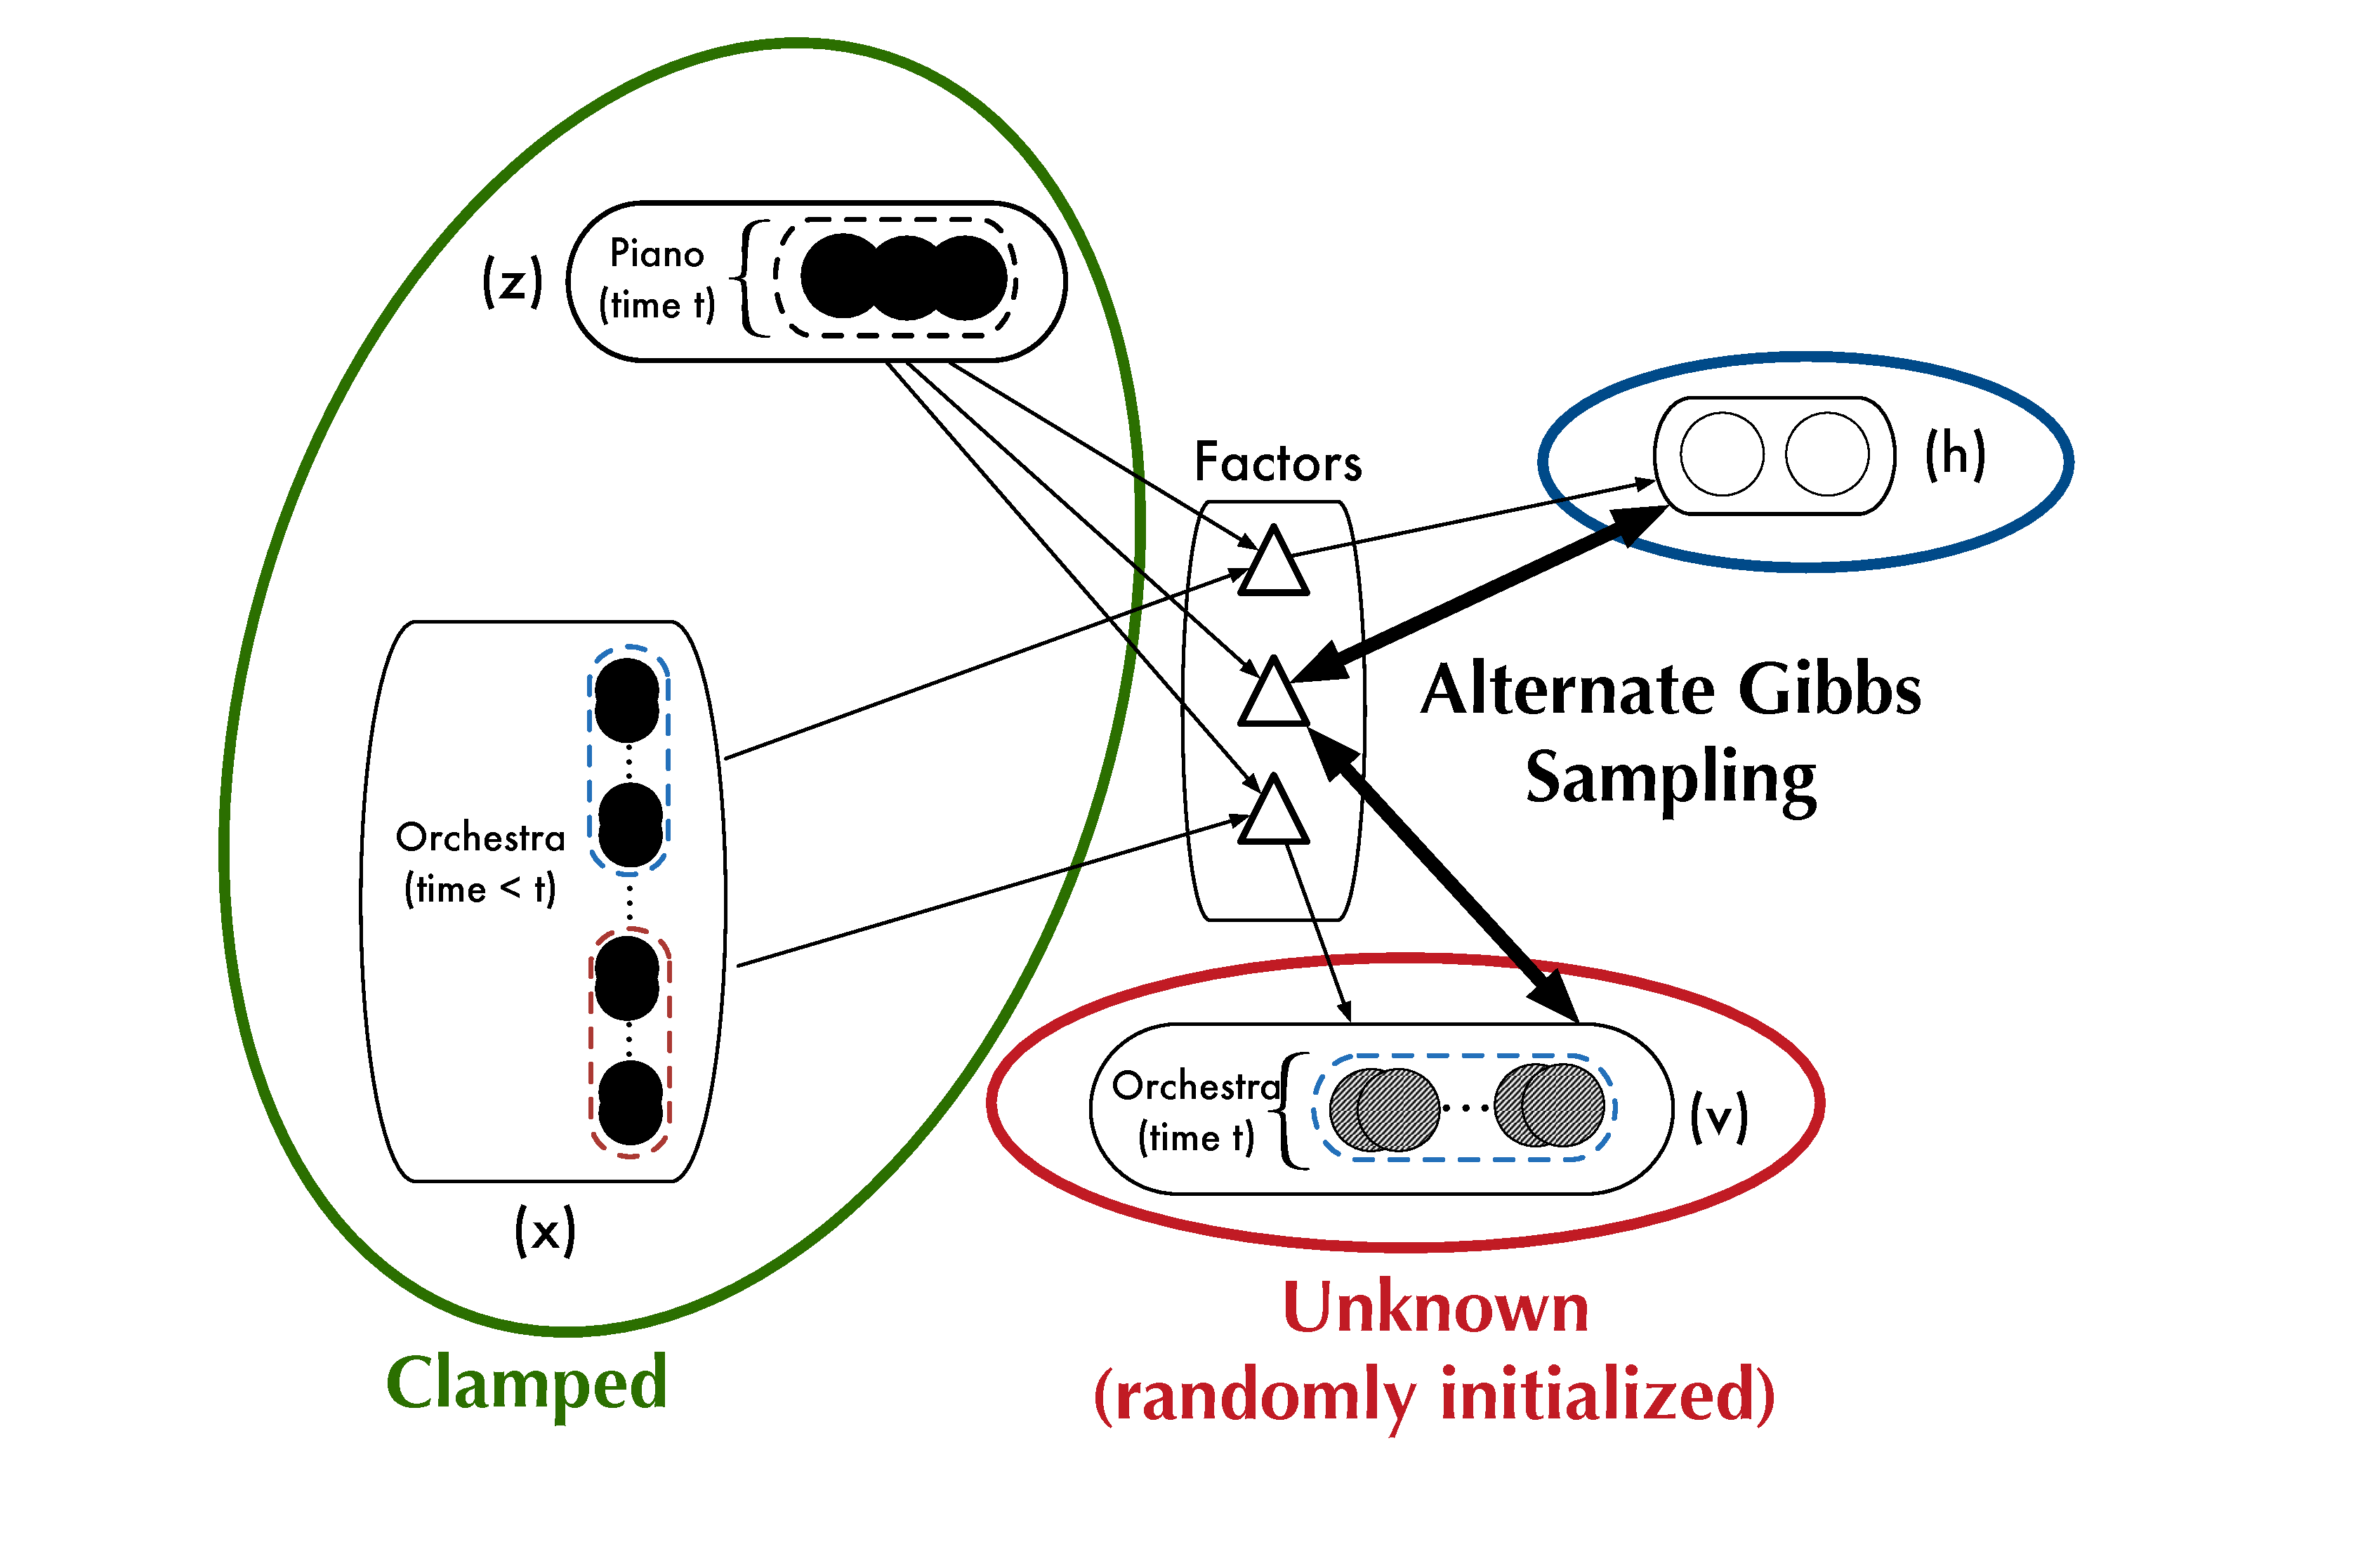
\includegraphics[scale=0.14]{FGCRBM_sampling}
\caption{\textit{Sampling in a FGCRBM}. Context and feature units are respectively clamped to the last ($t-1$ to $t-N$) orchestral frames and the current ($t$) piano frame. Visible units are randomly initialized. Then several Gibbs sampling step are performed until reaching the equilibrium distribution of the model (in our case 40).}
\label{fig:FGCRBM_sampling}
\end{figure}
% Role des unités conditionelles et tout le tralala dans les modèles
If correctly trained, the distribution of the model is supposed to be close (in the sense of the Kullback-Leibler divergence \cite{hinton2002training}) to the underlying probability distribution of the data. Therefore, by sampling from it, we are able to generate data \textit{similar} to the one observed in the training dataset yet unseen.
Sampling from a trained model means being able to draw samples from the marginal distribution of the visible units. This is impossible when the partition function is intractable, but alternate Gibbs sampling can be used. This sampling process is called the generative step and can be described as follows. After randomly setting the visible units (for each index $i$, $\bm{v}_{i} \sim \mathcal{U}(0,1)$), K Gibbs sampling steps are performed to obtain a visible sample. The objective of these K steps is to reach the equilibrium distribution of the model. Even though an theoretically  infinite number of steps is necessary, 20 to 100 steps are typically sufficient.

\section{Projective orchestration}
In this section, we introduce and formalize the automatic projective orchestration of a piano score as presented in \prettyref{fig:orch}. In particular, we detail our data representation, the evaluation framework, introduce the database used, and the results of different models in this framework.

\subsection{Data representation}
\label{sec:data_representation}
\begin{figure}
\centering
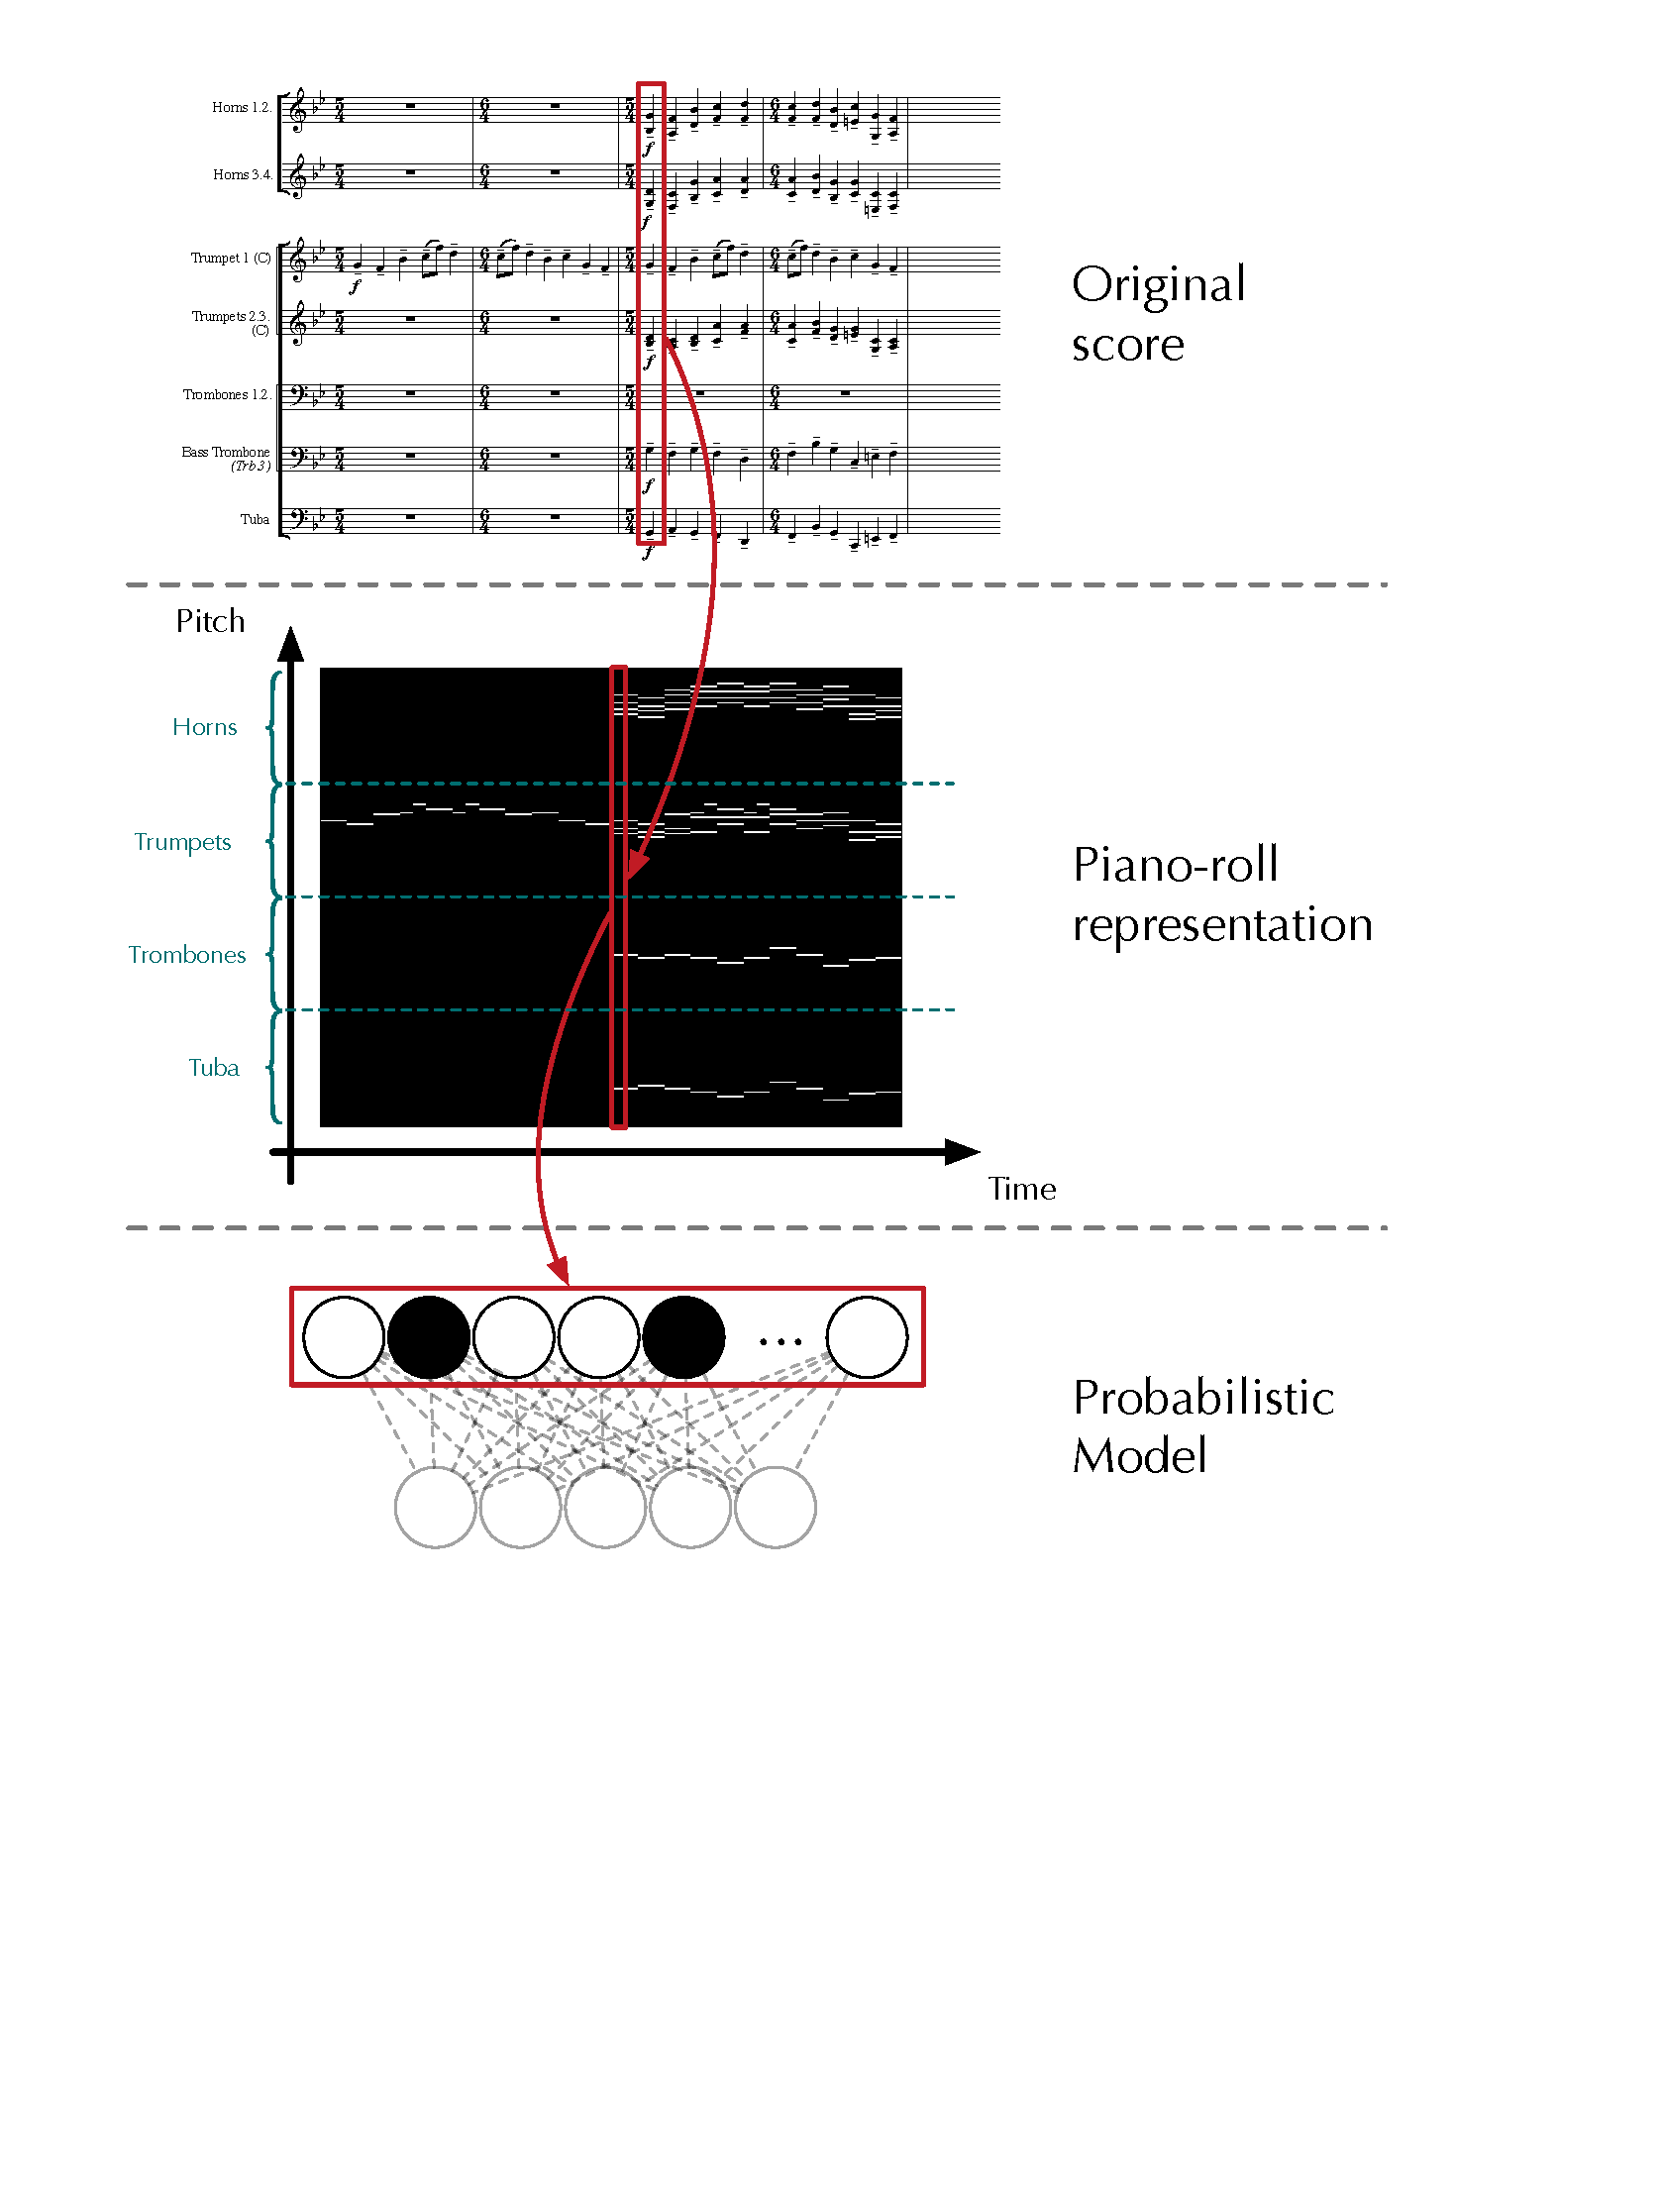
\includegraphics[scale=0.35]{data_representation}
\caption{The successive visible units of a neural network could be the successive temporal frames of a \textit{pianoroll}. A \textit{pianoroll} is a representation of musical events, discrete on both the frequency (pitch) and the time (frames) scales. For a single instrument, a pitch $p$ at time $t$ can be either played or not, which is represented by a one or zero in the \textit{pianoroll}. This definition is extended to an orchestra by simply concatenating the \textit{pianorolls} of each instruments along the pitch dimension. One can see on the figure that the same instruments are grouped together event if they don't play the same thing. For instance, trumpets 1, 2, 3 and 4 are grouped under one trumpet part, which then contains 4 voices chords.}
\label{fig:pianoroll}
\end{figure}
We used a data representation inspired by the \textit{piano-roll} representation traditionally used to model polyphonic music of a single instrument (see detailed on \prettyref{fig:pianoroll}). Piano and Orchestra data are represented in two different \textit{piano-roll}, then for the piano part a standard pianor-roll is used. The orchestra simply consists in the concatenation of the \textit{piano-roll} of each instrument along the pitch dimension. Note that the dynamic 	information is lost since we use binaries units which solely indicates if a note is on or off. In order to keep a reduced number of unit we systematically remove, for each instrument, any pitch for which is never played in the training database. By doing this on our database, we reduced the dimension of the orchestral vector from 2432 to 191 and the piano size went from 128 to 43.

Also, we follow the usual orchestral simplifications used when writing orchestral scores by grouping together all the instruments of a same section. For instance, the section \textit{violin 1}, composed by many instrumentalists (10 or more), is written as a single part.

Conditional models allow to generate sequences of data under a certain context. Projective orchestration can be seen as producing an orchestral score, conditionally on a piano score. In order to guarantee a form of temporal continuity in the orchestration, the recent past of the orchestral sequence is also added in the contextual information (see \prettyref{fig:pianoroll}). We kept 14 instruments among the one present in the database and discarded some very sparsely represented ones (\textit{e.g.} english horn, clarinet bass... by associating them to a close instrument. An exhaustive list of these approximations is given in annex (OAZDJOAZIDJOAZIDJ).

\begin{figure}
\centering
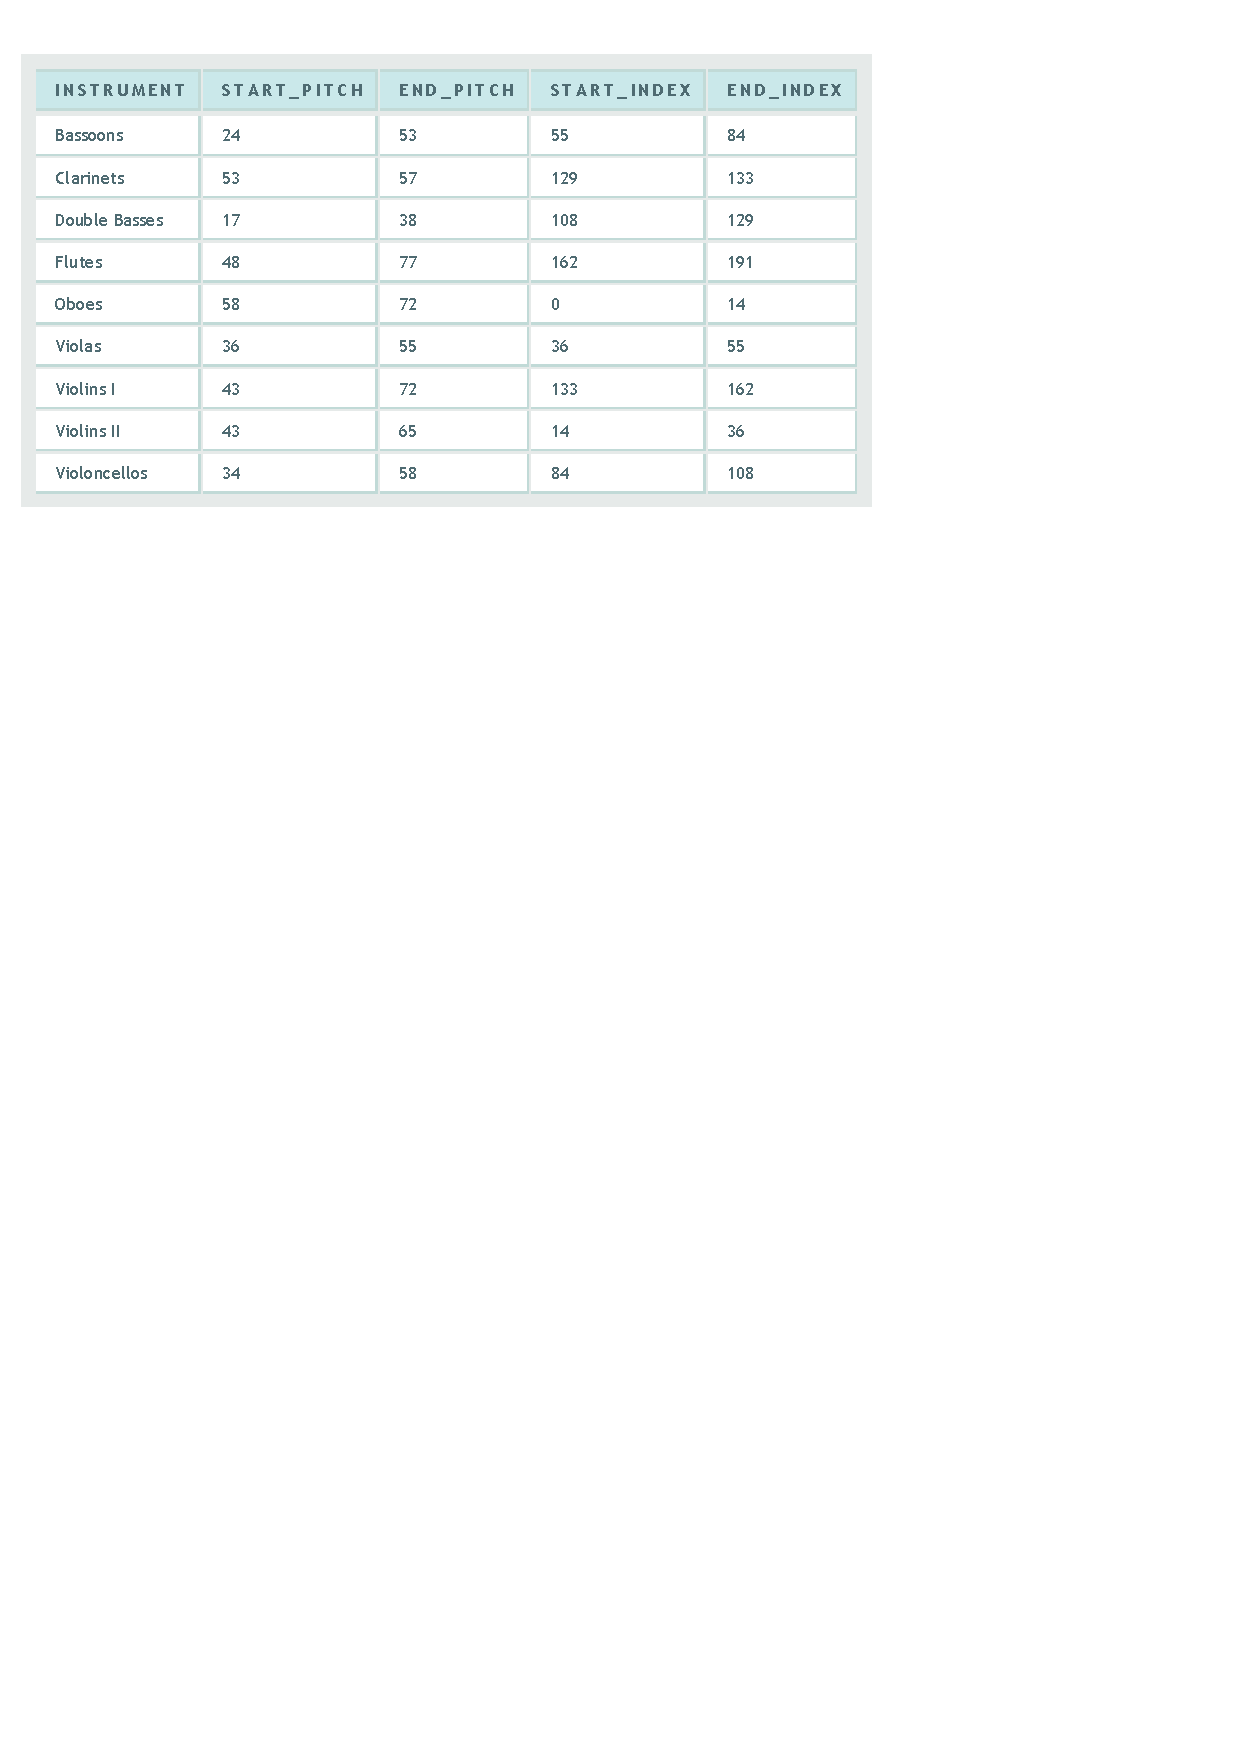
\includegraphics[scale=0.55]{orch_mapping.pdf}
\caption{Relation between indices in the reduced representation and real pitch for each instrument}
\label{fig:orch_mapping}
\end{figure}

For a piece of music, we define two multi-dimensional time series $Orch(t)$ and $Piano(t)$ with $t$ in $\left[ | 1 , N_{T} | \right]$ where $N_{T}$ is the lenght of the piece. Those are respectively defined by the sequence of column vector from the \textit{pianoroll} representation of the orchestra part and of the piano part.

At each time frame $t$, the visible units of the cRBM represent the current orchestral vector ($Orch(t)$), conditional units are used to model the influence of the past orchestral vectors $Orch(t-1) , ... , Orch(t-N)$ and the influence of the current piano frame ($Piano(t)$) over the visible units. The context units are then defined by the concatenation of the past orchestral frames and the current piano frame
$ Context(t) = \left[ Piano(t) , Orch(t-1) , ... , Orch(t-N)\right]$.

The \textit{FGcRBM} model allows to separate the influence of the current piano frame and the past orchestral frames. The current piano frame defines the feature units ($z$) 

$\text{Features}(t) = \text{Piano}(t)^{T}$

, and the concatenation of the past orchestral frames define the context units ($x$) 

$\text{Context}(t) = \left[ \text{Orch}(t-1)^{T} , ... , \text{Orch}(t-N)^{T} \right]^{T}$ 

(\prettyref{fig:FGCRBM}).

Note that we do not restrain the possible pitches of each instrument to the pitches seen in the piano score at each specific time frame. Indeed, orchestrating a piano score cannot be reduced to the simple repartition between the different instruments of the same notes already written in the piano score. Instead, the harmonic structure is often enriched by extra notes, ranging from simple octaviations to harmonic expansions (more complex chords with a specific colour). The melody might be doubled by several instruments at the unison, octave or even double octave.

\subsection{Database}
We used a parallel database of piano scores and their orchestration by famous composers. The database consists of 76 \textit{XML} files. Given the complexity of the distribution we wanted to model and the reduced size of the database we have accessed to, we decided to keep as a test dataset only the last half of one track from our database. Hence 75 and a half files were used to train our model. We chose to do so in order to have the best generation ability.
The contrastive-divergence algorithm has been applied on mini-batches of size $100$ during the training phase. Thus we obtained $335$ mini-batches for the frame-level measure, and $89$ for the event-level measure.
For each instrument, the pitch range is reduced to the \textit{tessitura} observed in the training dataset (\prettyref{sec:data_representation}). We used a rhythmic quantization of 8 frames per beat.

\subsection{Evaluation}
A objective criterion of the performances of a model is necessary. Not only to compare the different systems, but also to find the best set of hyper-parameter for a given model. To our best knowledge, there is no quantitative evaluation framework for automatic projective orchestration. We propose here a first attempt in order to fill this gap by defining a projective orchestration inference task. Given a test database composed by piano scores and orchestrations proposed by experts (famous composer), it consists at each time frame $t$ to generate an orchestral vector $\hat{Orch}(t)$ knowing the piano frame $Piano(t)$ and the recent past of sequence of orchestral vectors $Orch(t-1),... Orch(t-N)$. The predicted vector $\hat{Orch}(t)$ is then compared to the ground-truth $Orch(t)$ via an accuracy measure.

The best way for evaluating generative models is to compute the likelihood of a set of existing vector which are referred to as the test set. In the case of latent units based models, this likelihood has to be marginalized over the visible units. However we have seen that this quantity is intractable in a \textit{RBM}, \textit{cRBM} or \textit{FGcRBM} (\prettyref{eq:likelihood}).

A solution is to define an evaluation task. A task commonly used in the closely related field of automatic music generation is a short-term predictive task based on a frame-level accuracy measure \cite{DBLP:journals/corr/YaoCVDD15,boulanger2012modeling,lavrenko2003polyphonic}.

The frame-level accuracy of a model is defined as the mean value of the accuracies measured for each time frame of a testing set.
For each time frame, we try to predict the orchestral frame $\hat{\text{Orch}}(t)$ knowing the recent past $\text{Orch}(t-1),...,\text{Orch}(t-N)$ and the piano frame $\text{Piano}(t)$. The predicted frame is compared to the original frame $\text{Orch}(t)$ through an accuracy measure \cite{boulanger2012modeling,DBLP:journals/corr/YaoCVDD15} defined by :
\begin{equation}
\text{Accuracy}  = \frac{TP(t)}{TP(t) + FP(t) + FN(t)}
\label{eq:accuracy}
\end{equation}
where $TP(t)$ (true positives) is the number of notes correctly predicted (note on in the prediction and ground-truth). $FP(t)$ (false positive) is the number of notes predicted which are not in the original sequence (note on in the prediction, off in ground-truth). $FN(t)$ (false negative) is the number on unreported notes (note off in prediction, on in ground-truth). 
Note that instead of binary values, activation probabilities are used for the predicted samples in order to reduce the sampling noise. In the case this probability is intractable, one should sample many predicted frames for each time frame and compute the mean value of those samples.

\begin{figure}
\centering
\includegraphics[scale=1]{result_frame_level}
\caption{Result of different model for the frame-level}
\label{fig:result_frame_level}
\end{figure}

However we observed an important flaw in the measure: the performance of a model heavily rely on the time quantization chosen in the \textit{piano-roll} representation (see \prettyref{fig:result_frame_level}). This phenomenon doesn't occur for continuous data (\textit{e.g.} audio signal) where a higher frequency sampling rate is positively received as an increased amount of information. In our case, a very short time quantization would lead to learn a model which simply repeats the previous frames, since this is actually what is observed most of the time.

Hence, we propose a new evaluation framework based on the previous work in automatic composition and called \textit{event-level orchestral inference}. The same accuracy measure is used (\prettyref{eq:accuracy}), but evaluations occur at en event-level. Musical events occur when two successive vectors are different in the time series defined by the orchestral \textit{piano-roll}. Since the task is slightly different, the training phase has been consequently changed so that a model is trained only on new event frames.
In a projective orchestral context, this modification makes sense since the model does not have to learn a rhythmic structure which is already established by the piano score. The results are given in \prettyref{fig:result_event_level}

\begin{figure}
\centering
\includegraphics[scale=1]{result_event_level}
\caption{Result of the \textit{cRBM} and \textit{FGcRBM} models on an event-level orchestral inference task.}
\label{fig:result_event_level}
\end{figure}

\section{Live Orchestral Piano (LOP)}

We introduce in this section the \emph{Live Orchestral Piano} (LOP)
application, which is the first software able to provide a way to
compose music with a full classical orchestra in real-time by simply
playing on a MIDI piano. The goal of this framework is to rely on
the knowledge learned by the model introduced in the previous sections
in order to perform the projection from a piano melody to the orchestra.


\subsection{Workflow}

The software is implemented on a client/server paradigm. This choice
allows to separate the orchestral computation part from the interface
and sound rendering engine. That way, multiple interfaces can easily
be implemented. It should also be noted that separating the computing
and rendering on different computers, can allow to use high-quality
and CPU-intensive orchestral rendering plugins. This can allow a more
realistic orchestral rendering with heavy amounts of computation performed
while ensuring the real-time constraint on the overall system (preventing
degradation of the computing part). The complete implementation workflow
is presented in Figure~\ref{fig:Live-orchestral-piano}.

\begin{figure*}
\begin{centering}
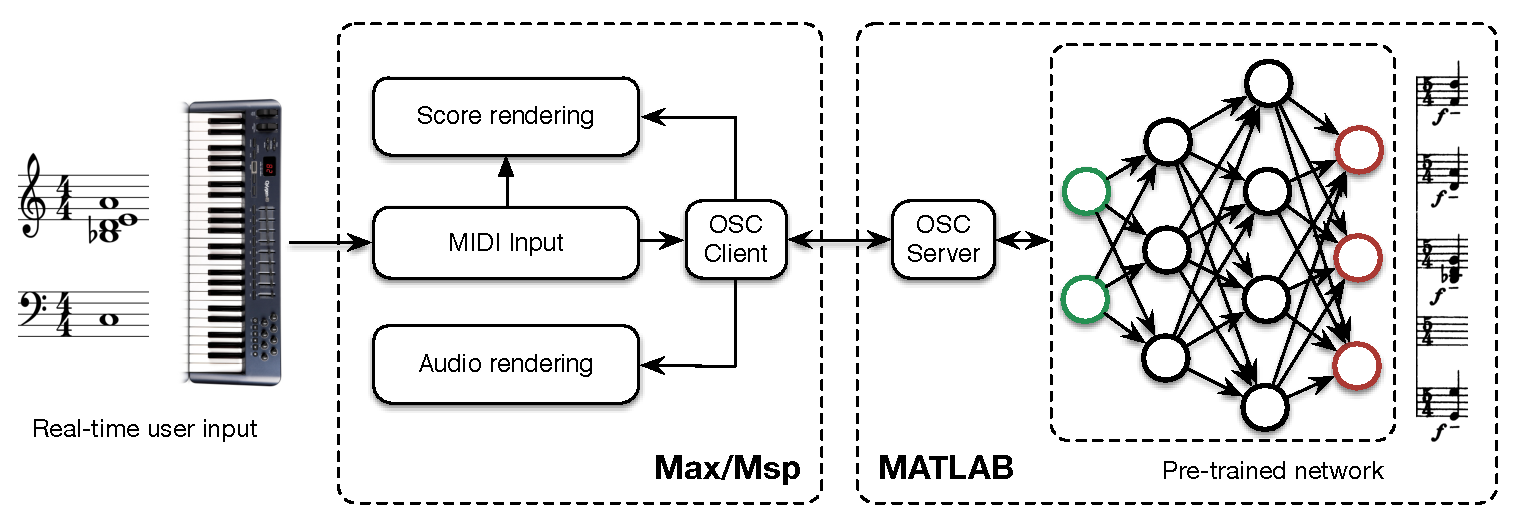
\includegraphics[scale=0.55]{workflow}
\par\end{centering}

\caption{\label{fig:Live-orchestral-piano}Live orchestral piano (L.O.P) implementation
workflow. The user inputs a melody which is transcribed into a score
and send via OSC from the Max/Msp client. Then, the MATLAB server
uses this vector of notes and process it following the aforementioned
techniques in order to obtain the orchestration. This information
is then sent back to Max/Msp which performs the real-time audio rendering }
\end{figure*}


As we can see, the user can input a melody (single notes or chords)
through a MIDI keyboard, which is retrieved inside the Max/Msp interface.
The interface transmits this symbolic information (as a variable-length
vector of active notes) via OSC to the MATLAB server. The interface
performs a real-time transcription of the piano score to the screen
in parallel. The server uses this vector of events to produce an 88
vector of binary input note activations (as defined in Section~\textbf{XXX}).
This vector is then processed by using the orchestration algorithms
presented in Section~\textbf{XXX} in order to obtain a projection
of a specific symbolic piano melody to the full orchestra (an operation
defined as \emph{projective orchestration}). The resulting orchestration
is then sent back to the client interface which performs both the
real-time audio rendering and score transcription. 

\textbf{NB: A good thing would be to compute the end-to-end latency
in the system ! And also to compute this with a variable number of
Gibbs steps ... all of this to show that we respect real-time constraints
/ requirements.}


\subsection{Interface}

The interface has been developed in Max/Msp, to facilitate both the
score and audio rendering aspects in a real-time environment. The
score rendering is handled by the \emph{Bach }library environment
\textbf{{[}INSERT REF{]}}. This interface provides a way to easily
switch between different orchestration models, while controling other
meta-parameters of the sampling. For instance the \emph{cutoff probability
}gives a direct access to the density of the generated orchestration
(in terms of number of played instruments). Indeed, a low cutoff probability
implies that most activation of notes will be taken into account in
the playback, while a high cutoff will produce more sparse orchestration.

\textbf{{[}INCLUDE FIGURE WITH LIVE EXAMPLE{]}}


\subsection{Examples\&}

Score and videos ?


\subsection{Offline generation}

Retry to generate full orchestral scores from piano scores. (with
new threshold and unit-variance transform) 

+ Assess various thresholds of generation

+ Try on Moussorgski and Beethoven







% We introduce an extension of this evaluation framework to an orchestral context through a task called \textit{frame-level orchestral inference}. This framework heavily relies on the previous works in automatic music generation and we discovered a bias in the measurement (dependency over the time quantization). Hence, we propose a new evaluation framework through a task called \textit{event-level orchestral inference} and present the results of the different models in it.
%
%
%
%\subsubsection{Frame-level accuracy}
%The frame-level accuracy of a model is defined as the mean value of the accuracies measured for each time frame of a testing set.
%For each time frame, we try to predict the orchestral frame $\hat{\text{Orch}}(t)$ knowing the recent past $\text{Orch}(t-1),...,\text{Orch}(t-N)$ and the piano frame $\text{Piano}(t)$. The predicted frame is compared to the original frame $\text{Orch}(t)$ through an accuracy measure \cite{boulanger2012modeling,DBLP:journals/corr/YaoCVDD15} defined by :
%\begin{equation}
%\text{Accuracy}  = \frac{TP(t)}{TP(t) + FP(t) + FN(t)}
%\label{eq:accuracy}
%\end{equation}
%where $TP(t)$ (true positives) is the number of notes correctly predicted (note on in the prediction and ground-truth). $FP(t)$ (false positive) is the number of notes predicted which are not in the original sequence (note on in the prediction, off in ground-truth). $FN(t)$ (false negative) is the number on unreported notes (note off in prediction, on in ground-truth). 
%
%Instead of binary values, activation probabilities are used for the predicted samples in order to reduce the sampling noise. In the case this probability is intractable, one should sample many predicted frames for each time frame and compute the mean value of those samples.
%
%\paragraph{Results}
%We evaluated the \textit{cRBM} and \textit{FGcRBM} previously presented \prettyref{sec:state_of_the_art} in both the frame-level and event-level frameworks. Those two models are compared to a random prediction of each frame and to a simple model that outputs the previous frame as the current frame prediction (i.e. a untrained 1 order linear predictor). The results are presented in \prettyref{fig:result_frame}. 
%We observed an important bias in the measurement : the performance of a model heavily rely on the time quantization chosen in the pianoroll representation. Those kind of phenomenon doesn't really occur for continuous data (\textit{e.g.} audio signal) where a higher frequency sampling rate is positively received as an increased amount of information. In our case, a very short time quantization would lead to learn a model which simply repeats the previous frames, since this is actually what is observed most of the time.
%
%We also present the result of those models on a purely predictive task for automatic music generation. Those results are only here for comparison purposes of the models in a well-established framework and to highlight the measurement bias. See \cite{boulanger2012modeling} for details about the evaluation framework and the \textit{RNN-RBM} model.
%
%\subsubsection{Event-level accuracy}
%A major flaw in the frame-level accuracy measure is its dependence to the rhythmic quantization chosen. Indeed, when the quantization become too small, it becomes highly probable that a frame is simply repeated at the next time frame. Hence, the best predictive model is simply a model which predict that the next time frame is the same as the frame $t-1$. This is not a desirable behaviour, and we propose an evaluation based on an event-level to address that issue.
%
%A musical event is defined as a change in the orchestral score, either a note being switched on or off. The predictive event-level accuracy measure relies on the same accuracy measure previously defined \prettyref{eq:accuracy}. The only difference is that it occurs at each new event instead of each new time frame. Since the task is slightly different, the training phase has been consequently changed so that a model is trained only on new event frames.
%
% Frame
% Event
%
% Precision et accuracy
%
% Séparer repeat et change true/false positive
%%%%%%%%%%%%%%%%%%\\
%%%%%%%%%%%%%%%%%%%%%%%%%%%\\
%%%%%%%%%\\
%%%%%%%%%%%%%%%%%%\\
% Coller une image
%\begin{figure}
%\centering
%\begin{tabular}{c c}
%\hline
%\multirow{2}{*}{Model} & Orchestral Frame-level (\%)\\
%\hline
%Random & 0.51\\ 
%Repeat & 93.25\\ 
%\hline \hline
%CRBM & 45.07\\ 
%FGCRBM & 2.05\\ 
%\end{tabular}
%\caption{Frame-level accuracy}
%\label{fig:result_frame}
%\end{figure}
%
%\begin{figure}
%\centering
%\begin{tabular}{c c}
%\hline
%\multirow{2}{*}{Model} & Orchestral Event-level (\%)\\
%\hline
%Random & 0.50\\ 
%Repeat & 93.25\\ 
%\hline \hline
%CRBM & 27.78\\ 
%FGCRBM & \\ 
%\end{tabular}
%\caption{Event-level accuracy}
%\label{fig:result_frame}
%\end{figure}
%% C'est de la merde, même le edvent-level ça règle pas du tout le problème : soit on prédit l'event mais avec un context basé sur les frames, et dans ce cas là le modèle repeat est bon, soit on prends que les event mais ça n'a aucun sens (pas de rythme...)
%%%%%%%%%
%%%%%%%%%
%%%%%%%%%\\
%%%%%%%%%
%%%%%%%%%\\


%\section{Live Orchestral Piano}

\section{Conclusion and future works}
% Better DB
% Change the data representation

% Acknowledgmentsinclude

% Bibliography
\bibliographystyle{iccc}
\bibliography{../Biblio/biblio}

\end{document}
